\documentclass[11pt]{article}

\usepackage{helvet}
\renewcommand{\familydefault}{\sfdefault}
\usepackage[onehalfspacing]{setspace}
\usepackage{ragged2e}
\justifying

\usepackage[margin=2.5cm]{geometry}
\usepackage{verbatimbox}

\usepackage[ngerman]{babel}

\usepackage{float}
\usepackage{wrapfig}
\usepackage{caption}
\usepackage{subcaption}

\usepackage{hyperref}

\usepackage{xcolor}
\definecolor{bx-green}{HTML}{398772}
\usepackage{graphicx}
\graphicspath{{./../pictures/}}
\usepackage{fancyhdr}
\renewcommand{\headrule}{{\color{bx-green}\rule[2ex]{\dimexpr\textwidth-3.55cm}{.95pt}}}
\setlength{\headheight}{30pt}
\usepackage{sectsty}
\sectionfont{\color{bx-green}}  % sets colour of sections
\subsectionfont{\color{bx-green}}


\begin{document}
\sloppy

\begin{titlepage}
    \color{bx-green}
    \vspace*{3cm}
        \centering
        \scalebox{3}{\textbf{Digitalisierung des internen}}\par
        \vspace{.5cm}
        \scalebox{3}{\textbf{Onboarding Prozesses}}\par
        \vspace{.5cm}
        \scalebox{3}{\textbf{neuer Mitarbeiter}}\par
        \vspace{5cm}
        \addvbuffer[0pt -.1cm] {
            
\includegraphics[width=\textwidth]{bx_logo.png}
        }
        {\LARGE \textbf{Benutzerdokumentation}}
    \vspace*{\fill}   
\end{titlepage}




\tableofcontents
\addtocontents{toc}{\protect\thispagestyle{empty}}
\pagenumbering{gobble}
\newpage
\pagenumbering{arabic}
\pagestyle{fancy}
\fancyhead[L]{Benutzerdokumentation - Julian Thiele}
\fancyhead[R]{
    \vspace*{-.4cm}
    
\includegraphics[height=.7cm]{bx_logo.png}
}

\section{Startseite}
Beim Aufrufen der Webseite gelangt der Nutzer auf die Login-Seite der Webanwendung.
Über den Login-Button kann der Nutzer sich mit seinem Microsoft-Account anmelden. Ist dieser auf dem Gerät bereits mit einem
Microsoft-Account angemeldet, wird die Anmeldung beim Betätigen des Buttons automatisch ausgeführt.

%=============================================
%               Login-Page
%=============================================

\begin{figure}[H]
    \centering
    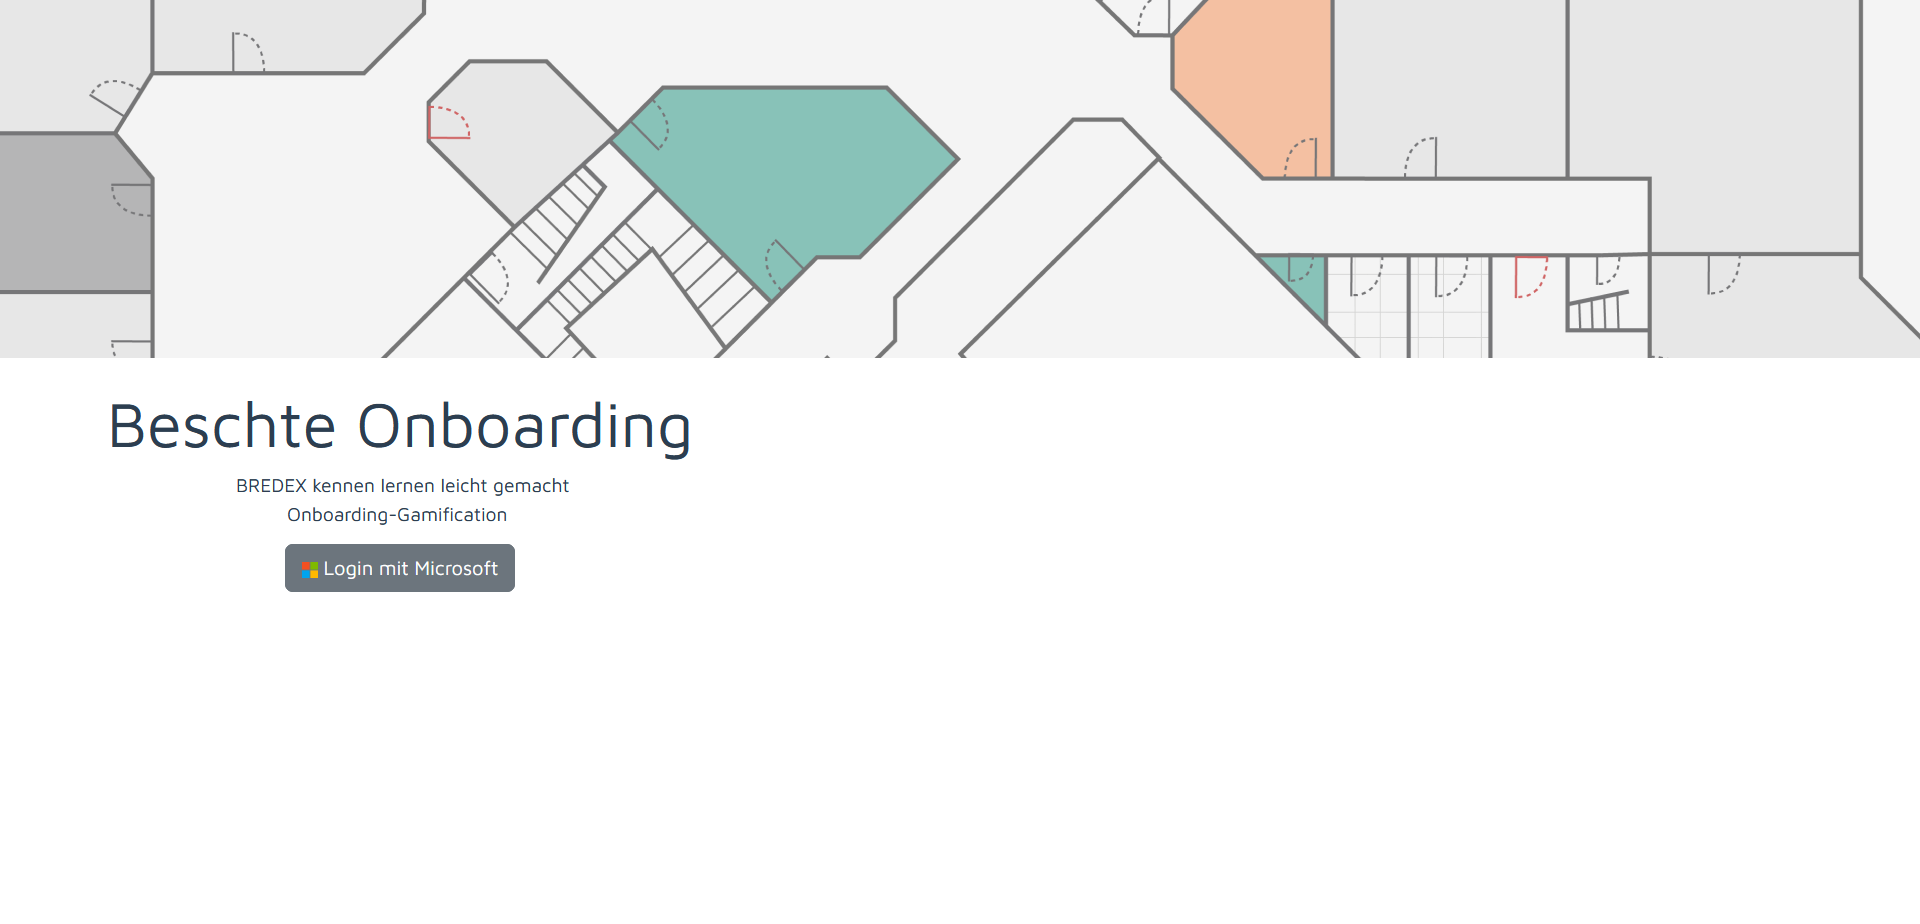
\includegraphics[width=\textwidth]{application/login_page.png}
    \caption{Login-Seite}
\end{figure}

\section{Allgemeiner Aufbau}

\subsection{Navigation}
Am oberen Rand der Anwendung befindet sich eine Navigationsleiste. Darüber können die verschiedenen Seiten der Anwendung erreicht werden.
% Die verschiedenen Seiten der Anwendung sind:
\begin{itemize}
    \item \textbf{Achievements: } Die Hauptseite der Anwendung. Hier können Achievements erledigt werden.
    \item \textbf{Rangliste: } Auf dieser Seite wird die Rangliste dargestellt, bei der man sich mit anderen Nutzern vergleichen kann.
    \item \textbf{Bearbeiten: } Hier können Achievement bearbeitet werden. Nur Personen mit Bearbeitungsberechtigung habe Zugriff auf diese Seite.
\end{itemize}
Der Bearbeiten-Tab ist nur für Nutzer sichtbar, die Zugriff auf diese Seite besitzen.
%=============================================
%               Navbar-Left/Right
%=============================================
% \begin{figure}[H]
%     \centering
%     \begin{subfigure}{0.5\textwidth}
%         \centering
%         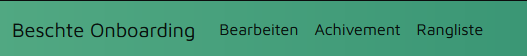
\includegraphics[height=.8cm]{application/navbar_left.png}
%         \caption{linke Seite}
%     \end{subfigure}
%     \hfill
%     \begin{subfigure}{0.3\textwidth}
%         \centering
%         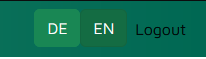
\includegraphics[height=.8cm]{application/navbar_right.png}
%         \caption{rechte Seite}
%     \end{subfigure}
%     \caption{Navigationsleiste}
% \end{figure}


Auf der rechten Seite der Navigationsleiste kann die Sprache der Anwendung zwischen Deutsch und Englisch umgestellt werden. Außerder kann sich der Nutzer dort
über der Ausloggen-Button aus des
\begin{figure}[H]
    \centering
    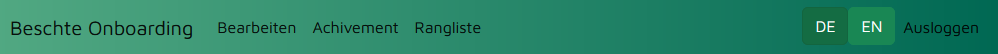
\includegraphics[width=\textwidth]{application/navbar.png}
    \caption{Navigationsleiste}
\end{figure}

\subsection{Hinweise}
Direkt unter der Navigationsleiste jeder Seite befindet sich eine kurze Beschreibung, was der Nutzer auf der jeweiligen Seite tun kann.

%=============================================
%               Hinweis
%=============================================
% \begin{figure}[H]
%     
\includegraphics[width=\textwidth]{application/description.png}
%     \caption{Beschreibung Achievementseite}
% \end{figure} ?

\section{Achievement Liste}
\subsection{Überblick}
Nach der Anmeldung wird der Nutzer auf die Achievement-Ansicht weitergeleitet. Achievements werden in 4 Zeitpunkte unterteilt:\newline
Erster Tag | Erste Woche | Erster Monat | Erstes halbes Jahr\newline
% \begin{itemize}
%     \item Erster Tag
%     \item Erste Woche
%     \item Erster Monat
%     \item Erstes halbes Jahr
% \end{itemize}
%=============================================
%               Sektions
%=============================================
\begin{wrapfigure}{r}{0.5\textwidth}
    \begin{center}
        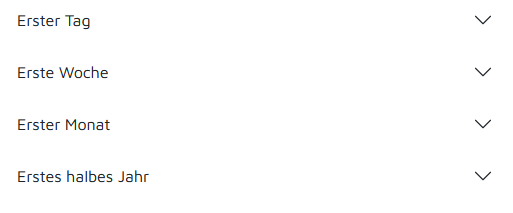
\includegraphics[width=0.4\textwidth]{application/sections.png}
    \end{center}
    \caption{Sektionen - Achievementseite}
\end{wrapfigure}

Je nach dem, wie lange der Nutzer bereits bei der BREDEX GmbH arbeitet, werden Achievements freigeschaltet. Ein Nutzer, der 
bereits seit einem Jahr bei BREDEX arbeitet, hat alle Sektionen freigeschaltet, währen einem Nutzer, der erst seit 2 Wochen bei BREDEX
arbeitet, nur die ersten beiden Abschnitte zur Verfügung stehen.
\clearpage
\subsection{Achievements erledigen}

Klappt der Nutzer eine Sektion aus, werden die Achievements dieses Zeitabschnittes angezeigt.
Jedes Achievement beinhält einen Text, der die Aufgabe des Achievements angibt. Darunter werden die Punkte angezeigt, die das jeweilige Achievement gibt.
Durch einen Klick auf den Button in dem Achievement kann dieses als erledigt markiert werden. Über denselben Button können bereits
erledigte Achievement wieder als nicht-erledigt markiert werden.
Erledigte Achievements werden in der Darstellung ausgegraut, um sie von nicht-erledigten unterscheiden zu können und nicht-erledigte Achievements hervorzuheben.

%=============================================
%               Achievement
%=============================================
\begin{figure}[H]
    \centering
    \begin{subfigure}{.4\textwidth}        
        
\includegraphics[width=\textwidth]{application/achievement_done.png}
        \caption{erledigt}
    \end{subfigure}
    \hfill
    \begin{subfigure}{.4\textwidth}
        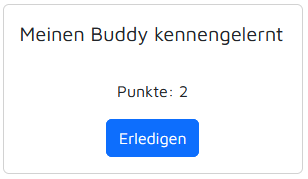
\includegraphics[width=\textwidth]{application/achievement_undone.png}
        \caption{nicht erledigt}
    \end{subfigure}
    \caption{Achievement}
\end{figure}


\subsection{Fortschrittsleiste}
Eine Leiste im oberen Teil der Ansicht zeigt dem Nutzer an, wie viele Achievements er bereits erledigt hat.
Ist die Leiste voll, sind alle Achievements erledigt, die dem Nutzer bereits verfügbar sind. 

%=============================================
%               Progress bar
%=============================================

\begin{figure}[H]
    \centering
    
\includegraphics{application/progress_bar.png}
    \caption{Fortschrittsleiste}
\end{figure}

\section{Rangliste}
Über die Navigation gelangt der Nutzer auf die Ansicht der Rangliste. 
Welche Nutzer in der Rangliste angezeigt werden, hängt von dem aktuell angemeldeten Nutzer ab.
Damit alle Nutzer in der Rangliste ungefähr ähnliche Vorraussetzungen haben, werden nur andere Nutzer angezeigt,
die höchstens einen Monat vor oder nach dem aktuell angemeldeten Nutzer bei der BREDEX GmbH angefangen haben.

\begin{figure}[H]
    \centering
    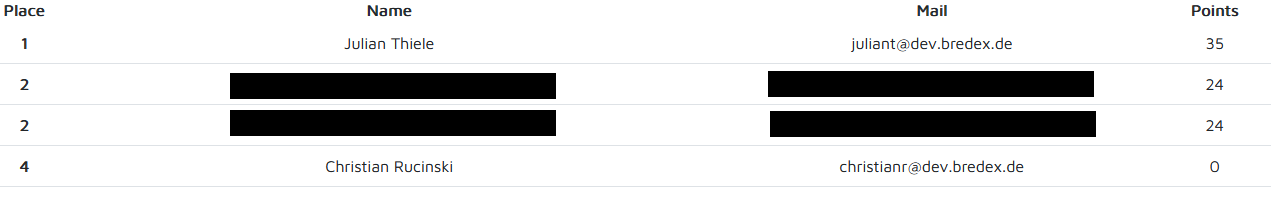
\includegraphics[width=\textwidth]{application/ranking_table.png}
    \caption{Rangliste}
\end{figure}
Die Nutzer werden in der Rangliste nach ihrer Platzierung absteigend sortiert. Je mehr Punkte ein Nutzer hat, desto besser ist seine Platzierung.
Die Punkte, die ein Achievement dem Nutzer einbringt, richtet sich nach der Schwierigkeit des Achievements und kann zwischen 0 und 5 Punken variieren.
Nutzer mit gleicher Punktzahl erhalten in der Rangliste dieselbe Platzierung.

%=============================================
%               Rangliste
%=============================================


\section{Management}
\subsection{Navigierung zur Management Seite}
Die Management Seite kann von Nutzern erreicht werden, denen es erlaubt ist Achievements zu bearbeiten. Der Link in der Navigationsleiste kann nur von jeweiligen
Nutzern gesehen werden.

\subsection{Achievements anlegen}
Auf der Management Seite sind die Achievements, ähnlich der Achievements Seite, in ihre Zeitabschnitte unterteilt.
Auf der rechten Seite eines jeden Zeitabschnittes kann auf einen Button mit einem "+" geklickt werden.
%=============================================
%               Anlegen Button
%=============================================
Im Anschluss dazu öffnet sich ein Modaldialog.
Über diesen Dialog können Achievements angelegt werden.

\begin{wrapfigure}{r}{.5\textwidth}
    \centering
    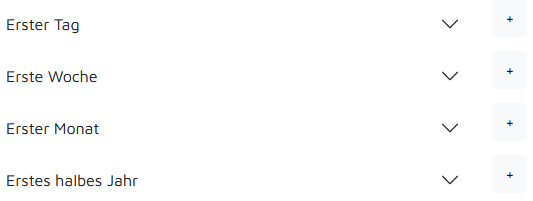
\includegraphics[width=.5\textwidth]{application/sections_manage.png}
    \caption{Sektionen bei Bearbeitung}
\end{wrapfigure}
%=============================================
%               Modal
%=============================================
Bei den ersten beiden Textfeldern muss der Nutzer die Aufgabe des Achievements eintragen.
Das erste der beiden Felder ist für den englischen, das Zweite für den deutschen Text.
Fehlt die Angabe in einem der beiden Textfelder, kann der Dialog nicht bestätigt werden.
Das Feld mit fehlender Angabe, wird dem Nutzer durch eine Eingabeaufforderung an dem Textfeld angezeigt.
\begin{figure}[H]
    \centering
    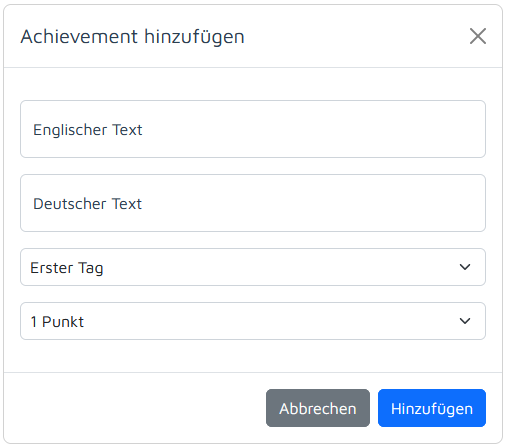
\includegraphics{application/popup_manage.png}
    \caption{Modaldialog}
\end{figure}

Im Anschluss kann der Zeitpunkt für die Freischaltung des Achievements ausgewählt werden.
Je nach dem, neben welchem Abschnitt der Nutzer auf den Button gedrückt hat, ist dieses Feld bereits
vorausgefüllt, kann aber über das Dropdown-Menü im Nachhinein geändert werden.

%=============================================
%               Dropdown
%=============================================

Final kann noch die Punktzahl des Achievements ausgewählt werden. Diese ist standardmäßig auf 1
gesetzt, kann aber über das Dropdown-Menü in einen Wert von 1 bis 5 geändert werden.

%=============================================
%               Punktzahl Dropdown
%=============================================
\begin{figure}[H]
    \begin{subfigure}{.5\textwidth}
        \centering
        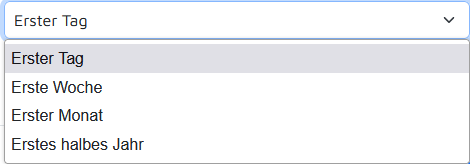
\includegraphics[height=3cm]{application/dropdown_time.png}
        \caption{Zeitabschnitt}
    \end{subfigure}
    \begin{subfigure}{.5\textwidth}
        \centering
        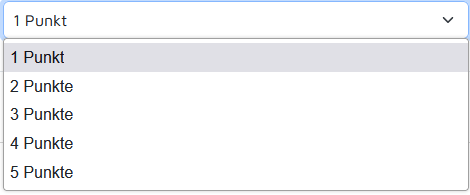
\includegraphics[height=3cm]{application/dropdown_points.png}
        \caption{Punkte}
    \end{subfigure}
    \caption{Dropdown Menüs}
\end{figure}

\subsection{Achievement bearbeiten}
Jedes Achievement kann über einen Button bearbeitet werden.
\begin{wrapfigure}{R}{.4\textwidth}
    \centering
    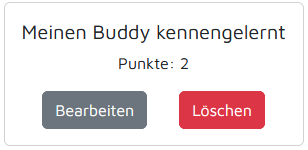
\includegraphics[width=.4\textwidth]{application/achievement_manage.png}
\end{wrapfigure}
Dieser Button befindet sich auf der Karte des Achievements.
%=============================================
%               Edit Button
%=============================================
Beim Drücken den Bearbeiten-Buttons, öffnet sich der selbe Dialog, der sich beim Erstellen eines neuen
Achievements öffnet. Der Dialog ist beim Bearbeiten mit den Daten des Achievements vorausgefüllt, das der Nutzer gerade
bearbeitet.

\subsection{Achievement löschen}
Neben dem Bearbeiten-Button existiert für jedes Achievement noch ein Button, um dieses zu löschen.
%=============================================
%               Delete Button
%=============================================
Versucht Nutzer ein Achievement zu löschen, öffnet sich ein Bestätigungsdialog, damit Achievements nicht aus versehen
gelöscht werden können.
%=============================================
%               Confirm Dialog
%=============================================





\end{document}